\chapter{Balanced Excitatory/Inhibitory Networks}
\label{ch:balanced-ei-networks}

\textit{Balanced networks are not quiet because nothing happens. They are
irregular because large excitation and large inhibition nearly cancel in the
mean, leaving the residual fluctuations and correlations to determine spiking.}

% ============================================================
\section{From Population Rates to Recurrent Input}
\label{sec:from-rates-to-input}
% ============================================================

Chapter~\ref{ch:single-neuron-population-models} defined spike trains and
population rates. A recurrent network closes the loop: population activity
creates synaptic input, and synaptic input changes future population activity.
For an excitatory/inhibitory (E/I) network, this loop has two signs. Excitatory
spikes push voltage upward; inhibitory spikes push it downward. A balanced
state occurs when both currents are large, but their sum is moderate.

Let $N_E^{\mathrm{tot}}$ and $N_I^{\mathrm{tot}}$ be the total numbers of
excitatory and inhibitory neurons, with
$N^{\mathrm{tot}}=N_E^{\mathrm{tot}}+N_I^{\mathrm{tot}}$. Later chapters use
$n_E,n_I$ for the number of neurons \emph{inside one cluster}; this chapter uses
the superscript ``tot'' whenever a class-wide count is meant. For a postsynaptic
neuron of type $\alpha\in\{E,I\}$, write the raw recurrent input as
%
\begin{equation}
  y_i^\alpha(t)
  =
  \sum_{j\in \mathrm{pre}_E(i)} J_{\alpha E}\,s_j^E(t)
  +
  \sum_{j\in \mathrm{pre}_I(i)} J_{\alpha I}\,s_j^I(t)
  + y_{\alpha}^{\mathrm{ext}}(t),
  \label{eq:ch04-ei-raw-input}
\end{equation}
%
where $J_{\alpha E}>0$ and $J_{\alpha I}<0$. The filtered current in the LIF
equation is $I_i^\alpha=\epsilon*y_i^\alpha$, using the same synaptic filter
as in \cref{eq:ch03-filtered-current}.

% ============================================================
\section{Mean Balance}
\label{sec:mean-balance}
% ============================================================

Suppose each postsynaptic neuron receives $K_{\alpha E}$ excitatory inputs and
$K_{\alpha I}$ inhibitory inputs, and suppose the stationary population rates
are $r_E$ and $r_I$. The stationary mean raw input is
%
\begin{keyequation}[Stationary E/I Mean Input]
\begin{equation}
  \bar y_\alpha
  =
  K_{\alpha E}J_{\alpha E}r_E
  +
  K_{\alpha I}J_{\alpha I}r_I
  +
  \bar y_{\alpha}^{\mathrm{ext}} .
  \label{eq:ch04-stationary-ei-mean-input}
\end{equation}
\tcblower
$K_{\alpha\beta}$: number of presynaptic neurons of type $\beta$ received by a
neuron of type $\alpha$; $J_{\alpha E}>0$ and $J_{\alpha I}<0$: excitatory and
inhibitory efficacies; $r_E,r_I$: stationary firing rates.
\end{keyequation}

\noindent In a balanced regime, the first two terms are individually large but
nearly cancel. If $K_{\alpha E}=fK$, $K_{\alpha I}=(1-f)K$,
$J_{\alpha E}=J$, and $J_{\alpha I}=-gJ$, then the recurrent contribution is
%
\begin{equation}
  JK\left[f r_E - g(1-f)r_I\right].
  \label{eq:ch04-simple-balance-condition}
\end{equation}
%
For comparable E and I rates, cancellation requires $g(1-f)r_I$ to be close to
$f r_E$, up to whatever external drive is needed to set the operating point.
The exact equality is not the point. The point is scaling: as $K$ becomes large,
a small mismatch between excitation and inhibition would create a large mean
current. Balanced activity therefore uses inhibitory feedback to keep the
residual input in the range where neurons fire irregularly but do not saturate.

The usual large-network scaling makes this statement sharper. If
$K_{\alpha\beta}=O(K)$ and
%
\begin{equation}
  J_{\alpha\beta}=\frac{j_{\alpha\beta}}{\sqrt{K}},
  \qquad
  \bar y_\alpha^{\mathrm{ext}}=\sqrt{K}\,i_\alpha^{\mathrm{ext}}+\bar y_{\alpha,0}^{\mathrm{ext}},
  \label{eq:ch04-balanced-scaling}
\end{equation}
%
then the leading $O(\sqrt{K})$ part of the mean input is
%
\begin{equation}
  \sqrt{K}
  \left[
    f j_{\alpha E}r_E
    +(1-f)j_{\alpha I}r_I
    +i_\alpha^{\mathrm{ext}}
  \right].
  \label{eq:ch04-leading-balance}
\end{equation}
%
A balanced asynchronous operating point requires the bracket to be small enough
that the remaining $O(1)$ current can sit near threshold. In numerical work this
is the practical ``balance solve'': choose baseline signed weights and external
drive so that the target rates give a modest residual mean, then study how
fluctuations and structured connectivity move the network around that point.

\begin{figure}[t]
\centering
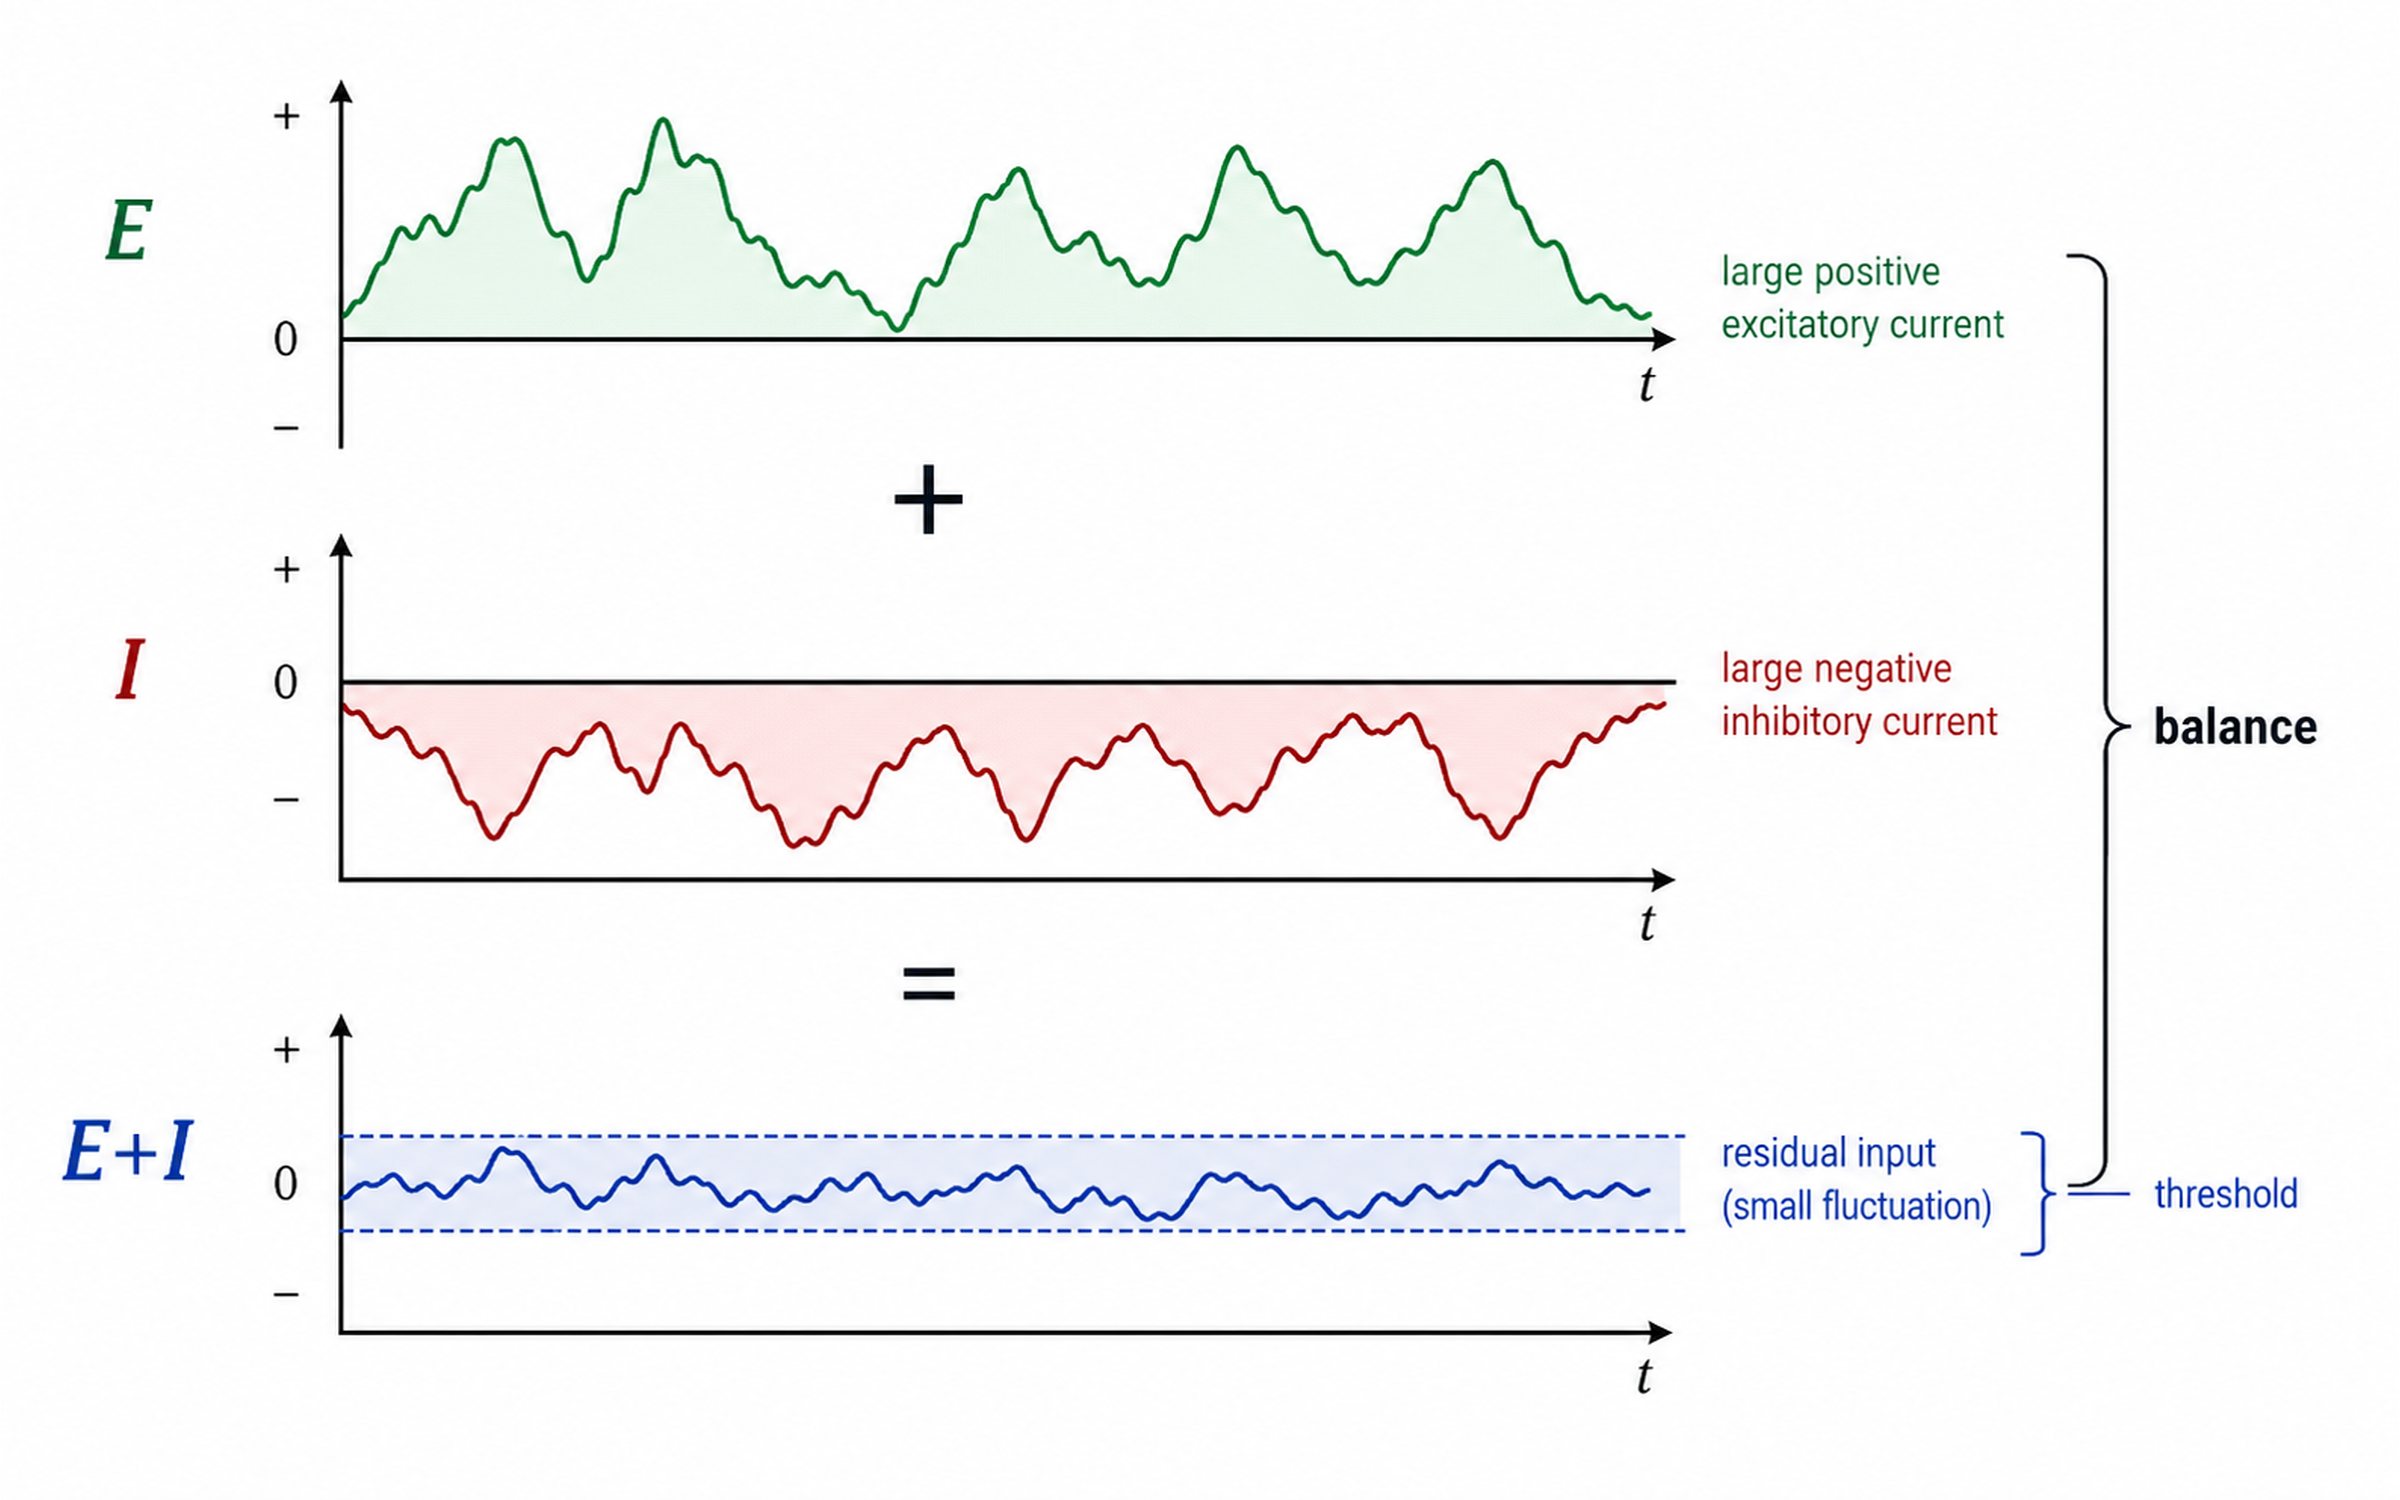
\includegraphics[width=0.92\textwidth]{figures/imagegen/ch04-balance-cancellation-img.png}
\caption{Balanced cancellation. Excitatory and inhibitory currents can be large
and structured while their sum remains near threshold. Once the mean cancels,
the residual fluctuations and correlations become the quantities that determine
irregular spiking and population-level variability.}
\label{fig:ch04-balance-cancellation}
\end{figure}

This is why balanced networks are a natural background for the roadmap. If the
mean input alone determined everything, clustered networks would reduce to a
static bookkeeping problem. Instead, the cancellation exposes second-order
objects: autocorrelations, cross-correlations, finite-size fluctuations, and
quenched variability in connectivity.

% ============================================================
\section{Sparse Random Connectivity with Fixed In-Degree}
\label{sec:sparse-fixed-indegree}
% ============================================================

Balanced networks are often sparse. Sparse does not only mean that the
connection probability is small; in the roadmap's subpopulation model it also
means that each postsynaptic population receives a fixed number of excitatory
source populations and a fixed number of inhibitory source populations. The
identities are random, but the counts are controlled.

Let $\Gamma_{ab}^{\alpha\beta}\in\{0,1\}$ indicate whether population
$(b,\beta)$ projects to population $(a,\alpha)$. For the external sources
$b\neq a$, fixed in-degree means
%
\begin{equation}
  \sum_{b\neq a}\Gamma_{ab}^{\alpha E}=K_E=fK,
  \qquad
  \sum_{b\neq a}\Gamma_{ab}^{\alpha I}=K_I=(1-f)K .
  \label{eq:ch04-fixed-indegree}
\end{equation}
%
The same-cluster excitatory and inhibitory populations are not part of these
external sums; they are the two local inputs handled separately below. This
differs from independent Erdos--Renyi sampling, where the in-degree itself
fluctuates. Fixed in-degree removes one source of variability so that the
remaining variability comes from which populations were selected and from the
spiking activity they generate.

A population-level fixed-indegree graph is generated row by row:
\begin{enumerate}
  \item For each target population $(a,\alpha)$, draw without replacement a set
  $S_{a\alpha}^E\subset\{b:b\neq a\}$ of size $K_E=fK$ and a set
  $S_{a\alpha}^I\subset\{b:b\neq a\}$ of size $K_I=(1-f)K$.
  \item Set $\Gamma_{ab}^{\alpha E}=1$ exactly for $b\in S_{a\alpha}^E$ and
  $\Gamma_{ab}^{\alpha I}=1$ exactly for $b\in S_{a\alpha}^I$; all other
  external entries are zero.
  \item Add the same-cluster E and I sources separately. If a microscopic
  neuron-level graph is also instantiated inside each selected source
  population, record whether the blocks are dense or use a fixed neuron
  in-degree $K_{\alpha\beta}^{\mathrm{cell}}$, because that choice sets the
  appropriate synaptic weight scaling.
\end{enumerate}

\begin{figure}[t]
\centering
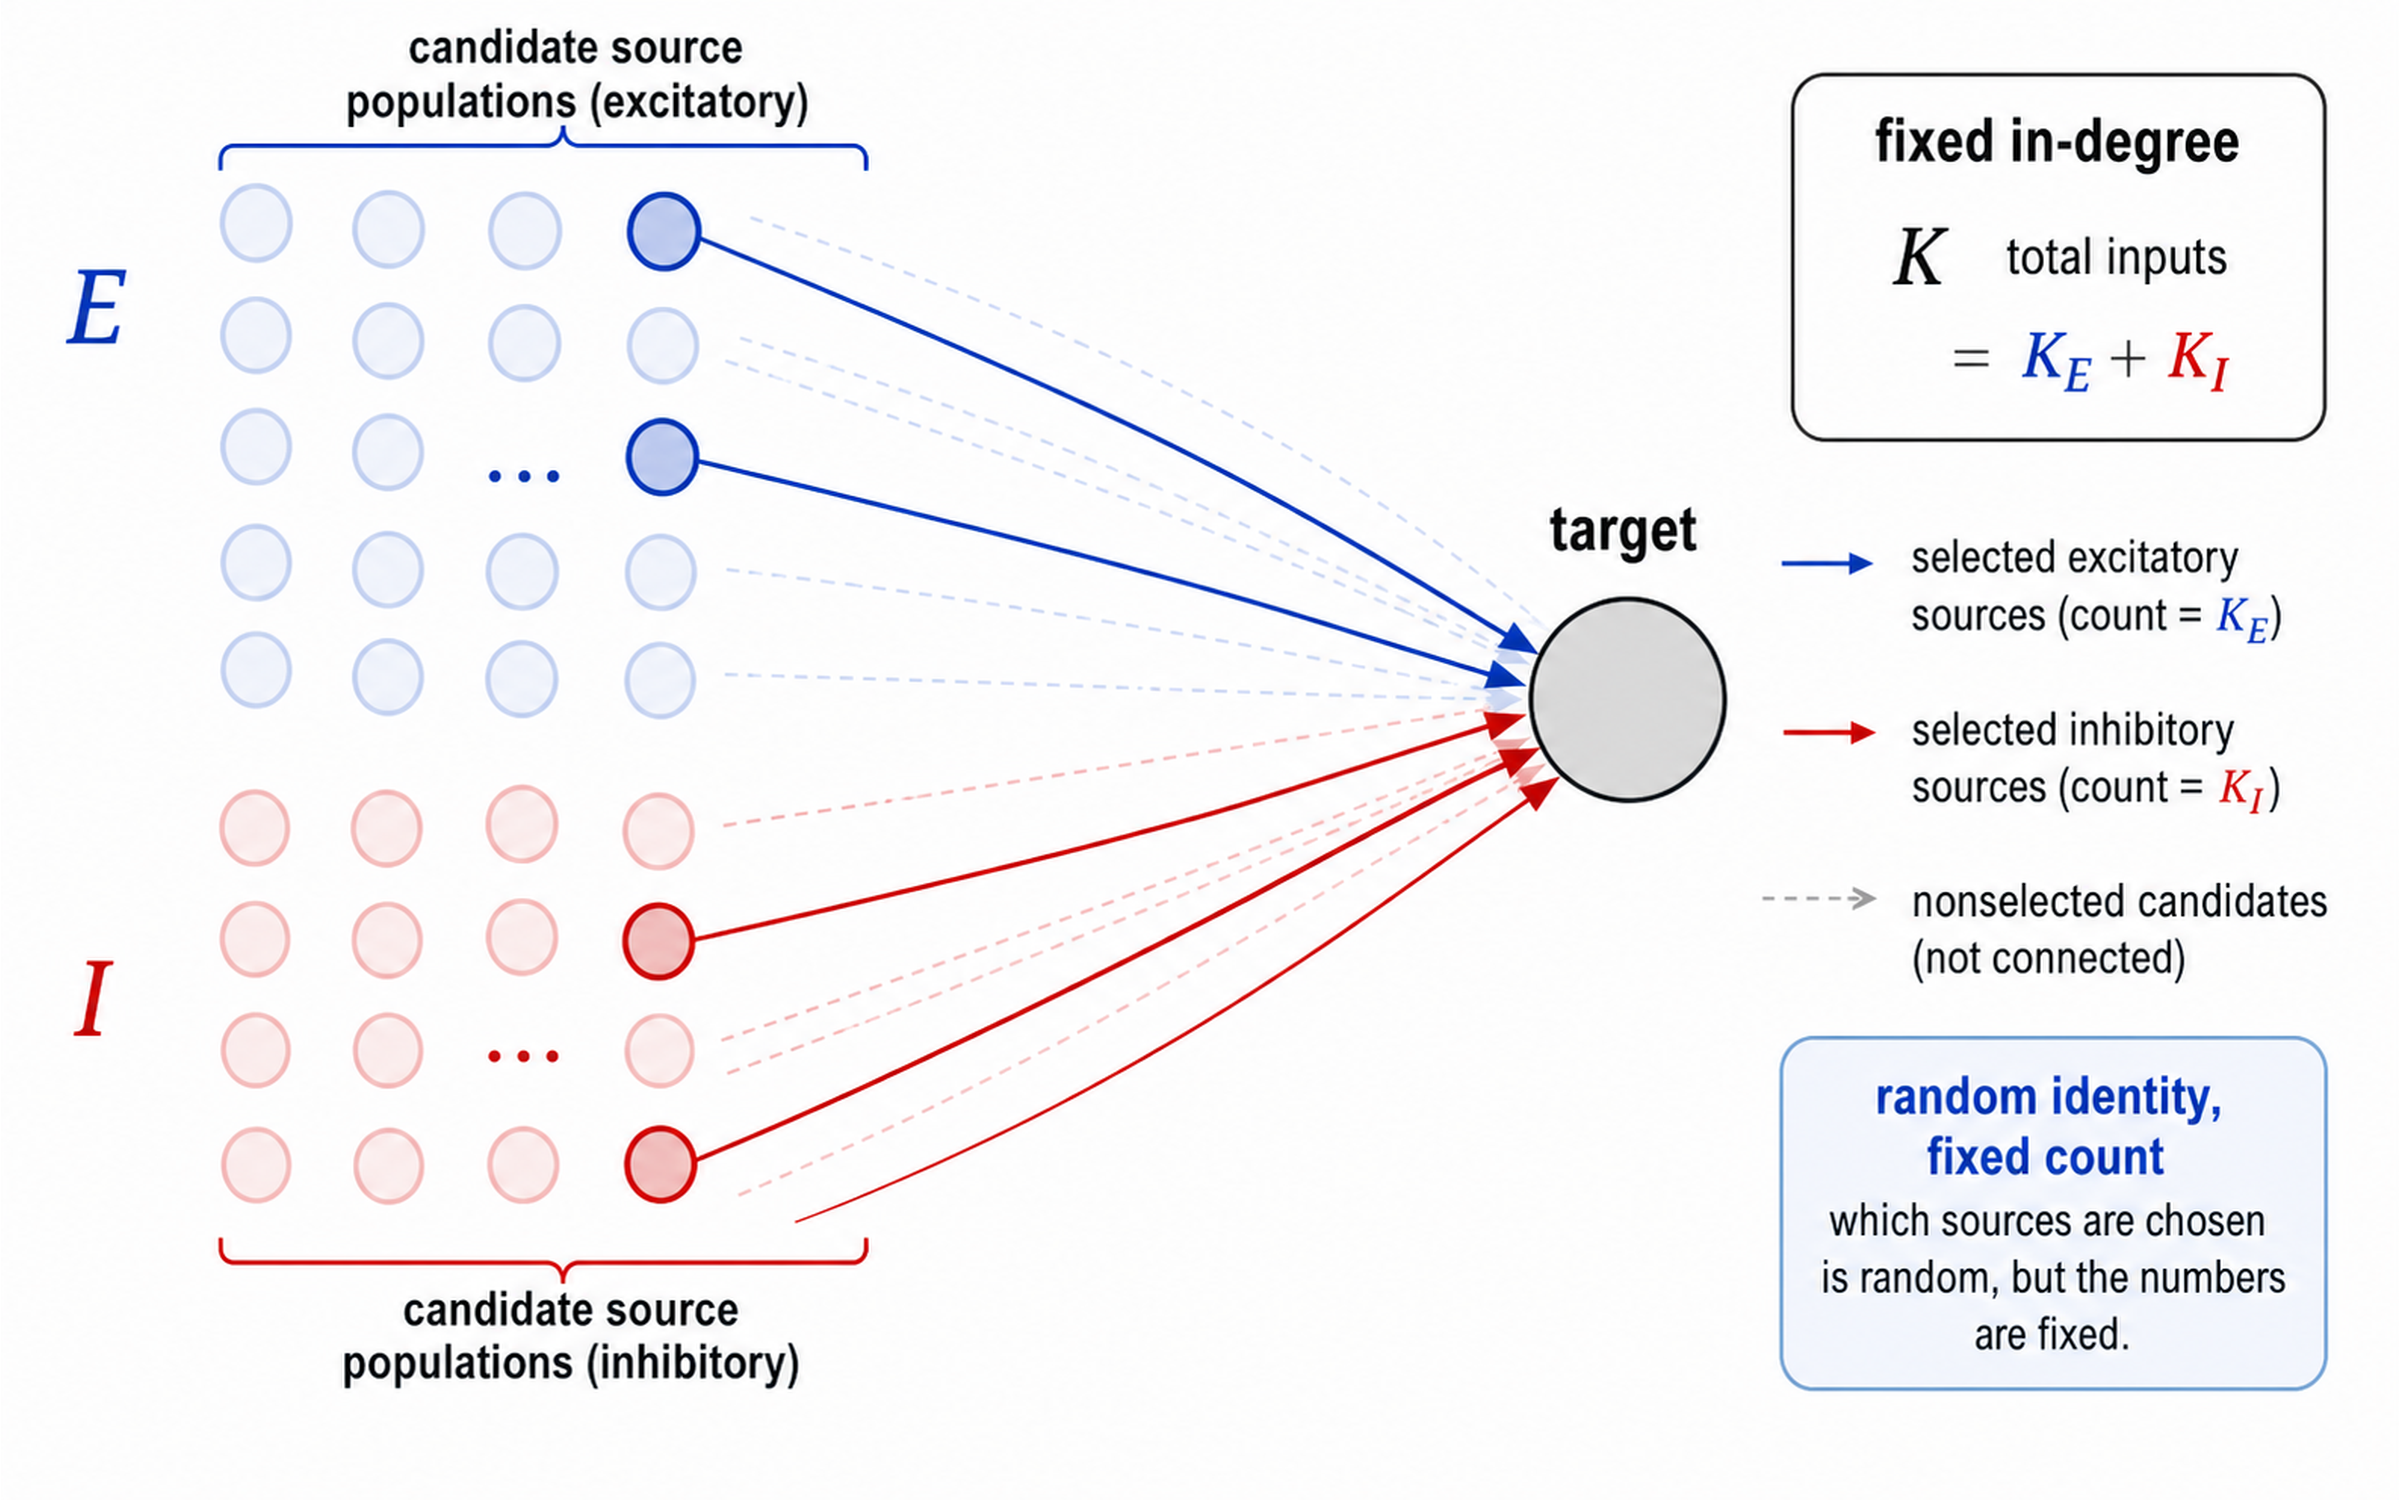
\includegraphics[width=0.90\textwidth]{figures/imagegen/ch04-sparse-fixed-indegree-img.png}
\caption{Sparse fixed-in-degree connectivity. A postsynaptic population receives
external inputs from exactly $K$ randomly chosen source populations, split into
$K_E=fK$ excitatory and $K_I=(1-f)K$ inhibitory sources. The random identities
create quenched structure, while the fixed count controls the mean input.}
\label{fig:ch04-sparse-fixed-indegree}
\end{figure}

For the rest of this sparse-subpopulation section, $n_E$ and $n_I$ denote the
numbers of excitatory and inhibitory neurons in one source population. For a
source population $b$, define
%
\begin{equation}
  A_b^E(t)=\frac{1}{n_E}\sum_{j=1}^{n_E}s_{b,j}^E(t),
  \qquad
  A_b^I(t)=\frac{1}{n_I}\sum_{j=1}^{n_I}s_{b,j}^I(t).
  \label{eq:ch04-subpopulation-activities}
\end{equation}
%
A simplified version of the roadmap's sparse subpopulation input is
%
\begin{align}
  y_a^\alpha(t)
  &=
  \hat J
  \left[
    \sum_{j=1}^{n_E}s_{a,j}^E(t)
    -
    g\sum_{j=1}^{n_I}s_{a,j}^I(t)
  \right]
  \notag\\
  &\quad
  +
  \check J
  \sum_{b\neq a}
  \left[
    \Gamma_{ab}^{\alpha E}\sum_{j=1}^{n_E}s_{b,j}^E(t)
    -
    \check g\,\Gamma_{ab}^{\alpha I}
    \sum_{j=1}^{n_I}s_{b,j}^I(t)
  \right],
  \label{eq:ch04-sparse-subpopulation-input}
\end{align}
%
where $\hat J$ weights within-population or within-cluster inputs and
$\check J$ weights inputs from other populations. The inhibitory factor
$\check g$ follows the roadmap convention
%
\begin{equation}
  \check g=\frac{f}{1-f}\,g .
  \label{eq:ch04-check-g-definition}
\end{equation}
%
With this rescaling, the external inhibitory contribution has the same
source-count normalization as the external excitatory contribution: the factor
$(1-f)K$ from the inhibitory source count cancels the denominator in
$\check g=fg/(1-f)$.

If all E and I subpopulations have the same stationary rate $r$, then the mean
input is obtained by averaging \cref{eq:ch04-sparse-subpopulation-input}:
%
\begin{align}
  \bar y
  &=
  \hat J(n_E-g n_I)r
  +
  \check J\left[fK n_E-\check g(1-f)K n_I\right]r
  \notag\\
  &=
  \bigl(\hat J+\check J fK\bigr)
  \bigl(n_E-g n_I\bigr)r .
  \label{eq:ch04-roadmap-balanced-mean}
\end{align}
%
matching the roadmap's balanced cancellation logic. The factor
$n_E-g n_I$ is the local E/I mismatch. The factor
$\hat J+\check J fK$ records how many sources contribute. Balance can be
achieved either by choosing inhibitory strength $g$ appropriately, by external
drive, or by recurrent feedback that adjusts $r_E$ and $r_I$.

% ============================================================
\section{Fluctuations After Cancellation}
\label{sec:fluctuations-after-cancellation}
% ============================================================

Once the mean has been controlled, the next object is the autocovariance of the
input,
%
\begin{equation}
  C_y^\alpha(\tau)
  =
  \left\langle
    \delta y_a^\alpha(t)\,
    \delta y_a^\alpha(t+\tau)
  \right\rangle,
  \qquad
  \delta y_a^\alpha(t)=y_a^\alpha(t)-\bar y_\alpha .
  \label{eq:ch04-input-autocovariance}
\end{equation}
%
This equation says exactly what is measured: subtract the stationary mean,
multiply the residual at two times separated by $\tau$, and average over time,
trials, or disorder realizations as appropriate.

In the large-$K$ sparse subpopulation regime, the sum over external source
populations dominates the within-population contribution. A schematic
large-$K$ simplification is
%
\begin{equation}
  C_y(\tau)
  \approx
  \check J^{\,2}
  \left[
    f n_E^2 + (1-f)\check g^{\,2}n_I^2
  \right]
  K\,C_A(\tau),
  \label{eq:ch04-large-k-covariance}
\end{equation}
%
where $C_A(\tau)$ is the autocovariance of a source population activity. The
inhibitory prefactor can be rewritten with
\cref{eq:ch04-check-g-definition}; it is shown in $\check g$ form to make the
fixed source counts visible. The lesson is robust: after mean cancellation, the
network is governed by how population activity fluctuates in time and how those
fluctuations are routed by the sparse graph.

This is the entry point for dynamic mean-field theory in later chapters. A
single population sees an effective fluctuating input whose autocovariance is
created by the activity of many other populations. Self-consistency then
requires the activity autocovariance produced by that input to equal the
$C_A(\tau)$ used to construct it.

% ============================================================
\section{Asynchronous Irregular Activity}
\label{sec:ai-activity}
% ============================================================

Balanced random networks often operate in an asynchronous irregular (AI)
regime. ``Irregular'' means that single-neuron spike trains have variable
interspike intervals, often roughly Poisson-like at coarse resolution.
``Asynchronous'' means that the population rate is comparatively steady because
neurons do not all spike together. The two properties are different: neurons can
be individually irregular while the population average remains smooth.

The AI state is not a lack of structure. It is a dynamical state in which
feedback suppresses coherent population oscillations and leaves each neuron
driven by fluctuating recurrent input. This makes it a useful baseline. Clustered
networks will be built by adding structured connectivity to this background and
asking when the structure creates active assemblies, switching, or chaos.

% ============================================================
\section{Inhibition-Stabilized Dynamics}
\label{sec:inhibition-stabilized}
% ============================================================

Inhibition-stabilized networks (ISNs) clarify the role of inhibitory feedback.
Consider a two-population rate linearization around a fixed point:
%
\begin{equation}
  \tau \frac{d}{dt}
  \begin{pmatrix}
    \delta r_E\\
    \delta r_I
  \end{pmatrix}
  =
  \left[
  -I_2+
  \begin{pmatrix}
    \phi_E' & 0\\
    0 & \phi_I'
  \end{pmatrix}
  \begin{pmatrix}
    w_{EE} & -w_{EI}\\
    w_{IE} & -w_{II}
  \end{pmatrix}
  \right]
  \begin{pmatrix}
    \delta r_E\\
    \delta r_I
  \end{pmatrix}.
  \label{eq:ch04-isn-linearization}
\end{equation}
%
Here $\delta r_E$ and $\delta r_I$ are small deviations of the excitatory and
inhibitory population rates from the fixed point, $I_2$ is the $2\times2$
identity matrix, and $\tau$ is an effective population time constant. The gains
$\phi_E'$ and $\phi_I'$ are the slopes of the excitatory and inhibitory transfer
functions at the operating point. The coefficient $w_{\alpha\beta}$ is the
effective strength from presynaptic population $\beta$ to postsynaptic
population $\alpha$; the minus signs in the inhibitory column encode that
inhibitory firing subtracts input current. In the language of
Chapter~\ref{ch:dynamical-systems-language}, the bracketed matrix divided by
$\tau$ is the Jacobian of the linearized rate flow, and the fixed point is stable
when all of its eigenvalues have negative real part.

The excitatory subnetwork alone is unstable if $-1+\phi_E'w_{EE}>0$. The full
E/I network can still be stable because an increase in $r_E$ recruits inhibition
through $w_{IE}$, and inhibition suppresses excitation through $w_{EI}$. In
that case inhibition is not merely damping an already stable excitatory system;
it is required for stability.

ISN logic will reappear in E/I clustered networks. Strong inhibitory pathways
can amplify the effect of quenched inter-cluster variability because inhibitory
feedback is the mechanism that holds the balanced state together. Perturbing
the inhibitory structure therefore changes not only a local current but also the
stabilizing loop itself.

\begin{figure}[t]
\centering
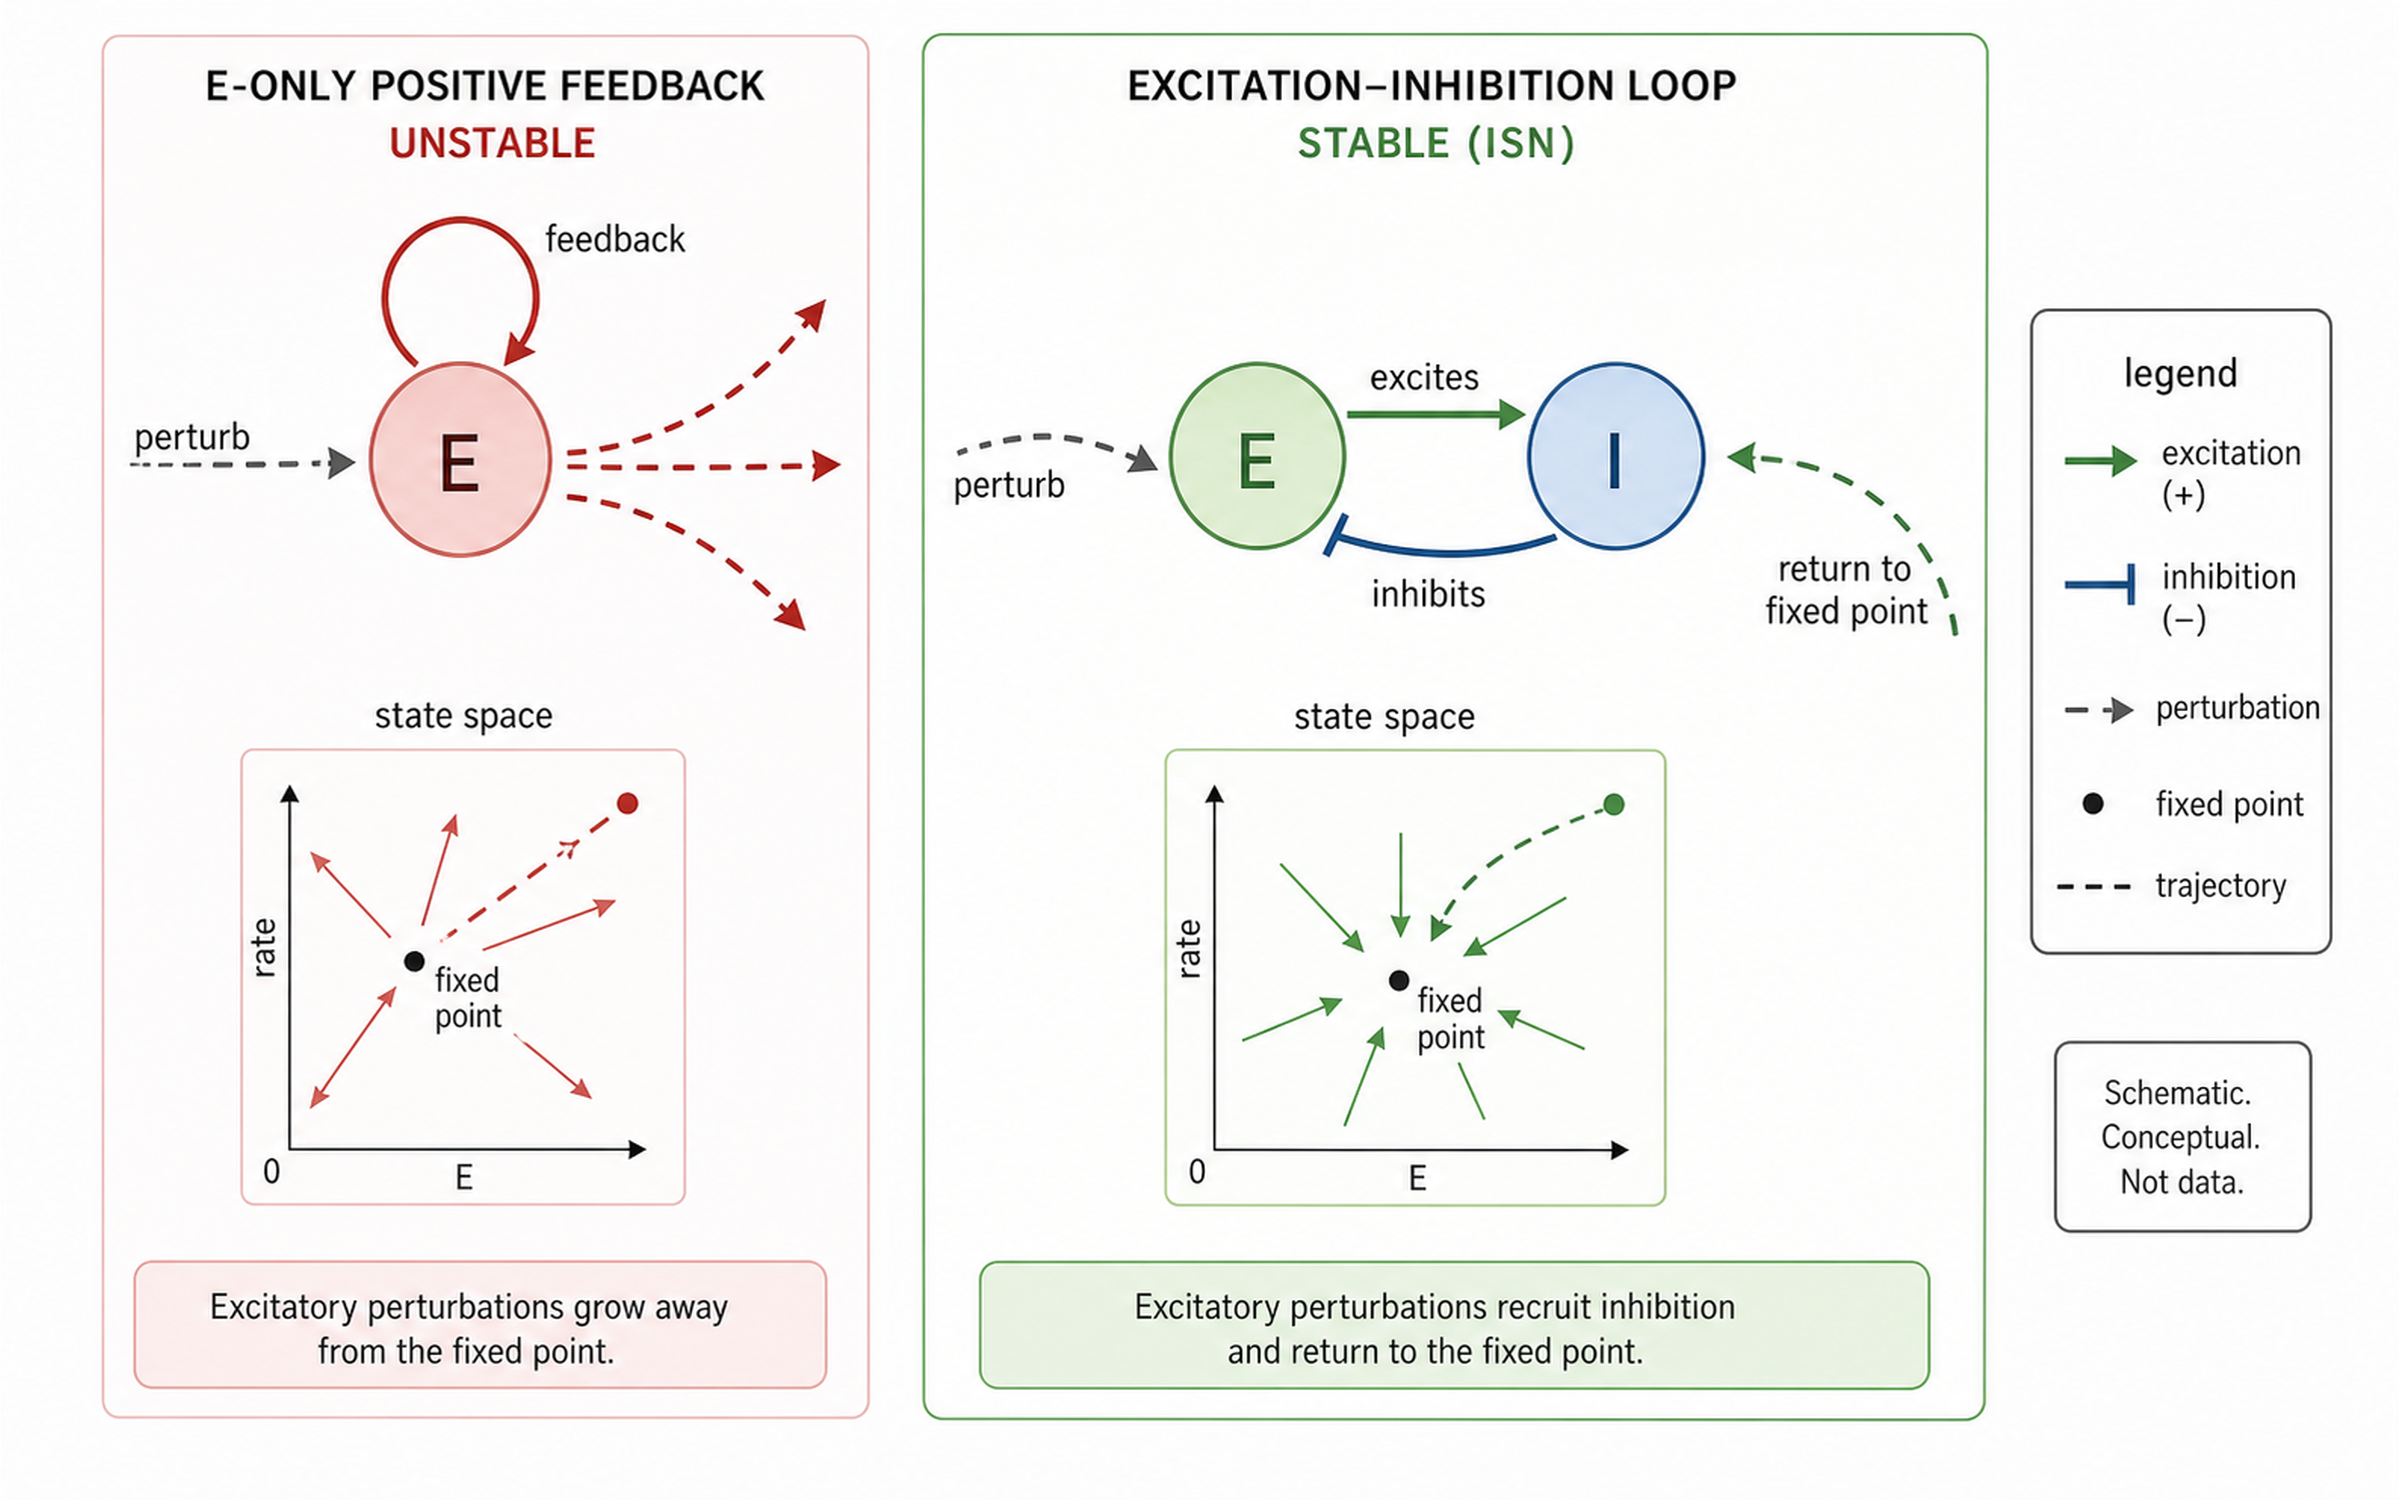
\includegraphics[width=0.90\textwidth]{figures/imagegen/ch04-inhibition-stabilized-loop-img.png}
\caption{Inhibition-stabilized feedback. The excitatory subnetwork can be unstable by itself when recurrent excitation overcomes leak, but the full E/I loop recruits inhibition through $w_{IE}$ and suppresses excitation through $w_{EI}$. In this regime inhibition is part of the stabilizing Jacobian, which is why changes to inhibitory structure can strongly reshape clustered dynamics.}
\label{fig:ch04-inhibition-stabilized-loop}
\end{figure}

\begin{chaptersummary}
\begin{center}
\renewcommand{\arraystretch}{1.45}
\begin{tabularx}{\textwidth}{@{}l X X@{}}
  \toprule
  \textbf{Concept} & \textbf{Equation} & \textbf{Key Point} \\
  \midrule
  Mean E/I input &
  $\bar y_\alpha=K_{\alpha E}J_{\alpha E}r_E+K_{\alpha I}J_{\alpha I}r_I+\bar y_\alpha^{\rm ext}$ &
  Large E and I terms must cancel to keep rates finite \\
  Balanced scaling &
  $J_{\alpha\beta}=j_{\alpha\beta}/\sqrt{K}$, $\bar y_\alpha^{\rm ext}=\sqrt K i_\alpha^{\rm ext}+O(1)$ &
  The leading $O(\sqrt K)$ current imposes the balance condition \\
  Fixed in-degree &
  $K_E=fK$, $K_I=(1-f)K$ &
  Random source identities with controlled source counts \\
  Population covariance &
  $C_y(\tau)=\langle\delta y(t)\delta y(t+\tau)\rangle$ &
  After mean balance, fluctuations become central \\
  Large-$K$ simplification &
  $C_y(\tau)\propto K C_A(\tau)$ &
  External sparse sources dominate second-order input statistics \\
  ISN stability &
  $-1+\phi_E'w_{EE}>0$ but full E/I Jacobian stable &
  Inhibition stabilizes an otherwise unstable excitatory loop \\
  \bottomrule
\end{tabularx}
\end{center}
\end{chaptersummary}

\begin{conceptquestions}
  \item In \cref{eq:ch04-stationary-ei-mean-input}, why can a small mismatch between
  excitation and inhibition become dangerous when $K$ is large?

  \item What is the difference between sparse fixed-in-degree connectivity and
  ordinary independent Erdos--Renyi connectivity?

  \item Why does balanced cancellation make autocorrelation functions more
  important rather than less important?

  \item Explain the terms ``asynchronous'' and ``irregular'' separately. Why
  can a population be asynchronous even when individual neurons spike
  irregularly?

  \item In an inhibition-stabilized network, what would happen to the
  excitatory subnetwork if inhibitory feedback were removed?
\end{conceptquestions}
